% \documentclass[aip,jcp,preprint,unsortedaddress,a4paper,onecolum]{revtex4-1}
\documentclass[aip,jcp,a4paper,reprint,onecolumn]{revtex4-1}
% \documentclass[aps,pre,twocolumn]{revtex4-1}
% \documentclass[aps,jcp,groupedaddress,twocolumn,unsortedaddress]{revtex4}

\usepackage[fleqn]{amsmath}
\usepackage{amssymb}
\usepackage[dvips]{graphicx}
\usepackage{color}
\usepackage{tabularx}
\usepackage{algorithm}
\usepackage{algorithmic}

\makeatletter
\makeatother

\newcommand{\recheck}[1]{{\color{red} #1}}
\newcommand{\redc}[1]{{\color{red} #1}}
\newcommand{\bluec}[1]{{\color{blue} #1}}
\newcommand{\vect}[1]{\textbf{\textit{#1}}}
\newcommand{\dd}{\textsf{d}}
\newcommand{\inv}{\textrm{inv}}

\newcommand{\mh}{\mathcal H}
\newcommand{\eps}{\varepsilon}
\newcommand{\ml}{\mathcal L}
\newcommand{\mt}{\mathcal T}
\newcommand{\mo}{\mathcal O}
\newcommand{\mi}{\mathcal I}
\newcommand{\mc}{\mathcal C}
\newcommand{\proj}{\mathit\Pi}
\newcommand{\fwg}{{\mathcal A}}
\newcommand{\bwg}{{\mathcal B}}
\newcommand{\bsigma}{\boldsymbol\sigma}


\begin{document}

\title{Linear response theory for core set identification}
\author{Han Wang}
\author{Carsten Hartmann}
\affiliation{Institute for Mathematics, Freie Universit\"at Berlin, Germany}
\author{Christof Sch\"utte}
\affiliation{Institute for Mathematics, Freie Universit\"at Berlin, Germany}
\affiliation{Zuse Institute Berlin (ZIB), Germany}
% \affiliation{Institute for Mathematics, Freie Universit\"at Berlin, Germany}

\date{\today}

\begin{abstract}
  % In this draft, we are trying to study the core set based Markov
  % State Model (MSM) under non-equilirbium conditions.
\end{abstract}

\maketitle

\section{Theoretical background}
\subsection{Classical equilibrium linear response theory}


In this section, we want to firstly give a brief description of the classical linear response
theory, for details see Ref.~\cite{tuckeman2010statistical} for
example.
We study the non-equilibrium system driven by some external force.
More strictly, we investigate the system that is governed by the
following Langevin equation:
\begin{align}\label{eqn:langevin-1}
  \dot{\vect q} & = \nabla_{\vect p}\mh(\vect q,\vect p), \\\label{eqn:langevin-2}
  \dot{\vect p} & =- \nabla_{\vect q}\mh(\vect q,\vect p)
  + \eps F_e(t) \vect D(\vect q) 
  - \gamma\vect p
  + \sigma\dot{\vect W}.
\end{align}
Here $\vect D$ is the external driving force applied to the system,
the magnitude of which is always assumed to be controllable.
$\eps F_e(t)$ is the strength of the driving as a function of time.
The prefactor $\eps$ indicates that we regard the driving force to be considerably smaller than the internal forces. We will comment on what is meant by "considerably smaller" further below.

% , and
% the magnitude of $F_e(t)$ is small and of order $\mo (\eps)$, $\eps \ll 1$.

Then the phase space distribution $f(\vect x, t)$ ($\vect x = \{\vect
q, \vect p\}$) is subject to the Kolmogorov forward equation:
\begin{align}\label{eqn:orig-forward}
  \frac{\partial}{\partial t} f(\vect x, t) - \fwg^\beta(t) f(\vect x, t) = 0
\end{align}
where $\fwg^\beta(t)$ is the forward infiniesimal generator given by
\begin{align}
  \fwg^\beta(t) =
  \frac{\sigma^2}2\Delta_{\vect p}
  - \nabla_{\vect p}\mh 
  \cdot\nabla_{\vect q}
  - \Big(
  -\nabla_{\vect q}\mh +
  \eps F_e(t)  \vect D  - \gamma\vect p
  \Big)\cdot\nabla_{\vect p}
  + 3N\gamma,
\end{align}
and $\beta2=\gamma / \sigma^2$ is the inverse temperature.
The equilibrium system
is governed by
the standard Langevin equation, i.e. with
vanishing driving force $\eps = 0$ in
Eqn.~\eqref{eqn:langevin-1} and \eqref{eqn:langevin-2}.

Under our smallness assumption on the driving force the full phase space distribution has the following asymptotic expansion in $\eps$:
\begin{align}\label{eqn:f-expan}
  f(\vect x, t) &= f_0(\vect x, t) + \eps f_1(\vect x, t)
  +\eps^2 f_2(\vect x, t) + \mo (\eps^3),
\end{align}
where $f_0=f_0(x,t)$ denotes the evolution of the phase space distribution for the undriven system (with $\eps=0$).
In addition we have:
\begin{align}\label{eqn:A-expan}
  \fwg^\beta(t) = \fwg^\beta_0 + \eps\fwg_1(t),
\end{align}
where
\begin{align}
  \fwg_0^\beta =&
  \frac{\sigma^2}2\Delta_{\vect p}
  -
  \nabla_{\vect p}\mh\cdot\nabla_{\vect q}
  - \big(
  -\nabla_{\vect q}\mh - \gamma\vect p
  \big)\cdot\nabla_{\vect p}
  + 3N\gamma,\\
  \fwg_1(t) =&
  - F_e(t)  \vect D \cdot\nabla_{\vect p}.
\end{align}

The invariant measure of $\fwg^\beta_0$ satisfies $\fwg^\beta_0f^\beta_{\inv}(\vect x) = 0$, and is given by the Boltzmann distribution
\begin{align}
  f^\beta_{\inv}(\vect x) \propto e^{-\beta\mh(\vect x)}
\end{align}
Inserting \eqref{eqn:f-expan} and \eqref{eqn:A-expan} into
\eqref{eqn:orig-forward}, 
the Kolmogorov forward equation becomes:
\begin{align}
  \frac{\partial}{\partial t}
  [f_0(\vect x, t) + \eps  f_1(\vect x, t) + \eps^2f_2(\vect x, t)]
  -
  [\,\fwg^\beta_0 + \eps\fwg_1(t)\,]
  [f_0(\vect x, t) + \eps  f_1(\vect x, t) + \eps^2f_2(\vect x, t)]
  = 0
\end{align}
Matching this equation at different orders of $\eps$, the zeroth
order gives:
\begin{align}\label{eqn:e-o0}
  \bigg[
  \frac{\partial}{\partial t}
  - \fwg_0^\beta
  \bigg]
  f_0(\vect x, t)
  = 0
\end{align}
which is the Kolmogorov forward equation of the undriven system. Matching the first and the second order gives:
\begin{align}\label{eqn:e-o1}
  \bigg[
  \frac{\partial}{\partial t}
  - \fwg_0^\beta
  \bigg]
  f_1(\vect x, t)
  =&
  \fwg_1(t) f_0(\vect x, t)\\\label{eqn:e-o2}
  \bigg[
  \frac{\partial}{\partial t}
  - \fwg_0^\beta
  \bigg]
  f_2(\vect x, t)
  =&
  \fwg_1(t) f_1(\vect x, t)
\end{align}
Formally solving \eqref{eqn:e-o0} -- \eqref{eqn:e-o2} with
initial conditions $f_1(\vect x, 0) = 0$ and $f_2(\vect x, 0) = 0$
gives
\begin{align}\label{eqn:f0-0}
  f_0(\vect x, t)
  =&\,
  e^{t\fwg^\beta_0}f_0(\vect x, 0) \\\label{eqn:f1-0}
  f_1(\vect x, t)
  =&\,
  \int_0^t\dd s\,
  e^{(t-s)\fwg^\beta_0}\circ
  \fwg_1(s) f_0(\vect x,s)
  =
  \int_0^t\dd s\,
  e^{(t-s)\fwg^\beta_0}\circ
  \fwg_1(s)\circ
  e^{s\fwg^\beta_0}f_0(\vect x, 0) \\\nonumber
  f_2(\vect x, t)
  =&\,
  \int_0^t\dd s\,
  e^{(t-s)\fwg^\beta_0}\circ
  \fwg_1(s) f_1(\vect x,s) \\\label{eqn:f2-0}
  &=
  \int_0^t\dd s
  \int_0^s\dd u\,\,
  e^{(t-s)\fwg^\beta_0}\circ
  \fwg_1(s)\circ
  e^{(s-u)\fwg^\beta_0}\circ
  \fwg_1(u)\circ
  e^{u\fwg^\beta_0}
  f_0(\vect x, 0) 
\end{align}
If the initial distribution is the invariant distribution, i.e.
$f_0(\vect x, 0) = f_{\inv}^\beta(\vect x)$,
\eqref{eqn:f0-0} becomes:
\begin{align}
  f_0(\vect x, t) = f_{\inv}^\beta(\vect x)
\end{align}
It can be shown that
\begin{align}
  \fwg_1(s) f_{\inv}^\beta(\vect x)
  =
  -\beta {F_e(s)}
  j(\vect x)
  f_{\inv}^\beta(\vect x),
\end{align}
where the \emph{dissipative flux} $j(\vect x)$ is defined by,
\begin{align}
  j(\vect x) =
  -\vect D\cdot\nabla_{\vect p}\mh
\end{align}
Then $f_1(\vect x, t)$ becomes:
\begin{align}
  f_1(\vect x, t)
  =
  -\beta
  \int_0^t\dd s\,
  F_e(s)\,
  e^{(t-s)\fwg^\beta_0}
  \big[
  j(\vect x)
  f_{\inv}^\beta(\vect x)
  \big]
\end{align}
Therefore, the linear order approximation to
the solution of~\eqref{eqn:orig-forward} is 
\begin{align}\label{eqn:solv-orig-linear}
  f(\vect x, t) =
  f_{\inv}^\beta(\vect x)
  - \eps\beta
  \int_0^t\dd s\,
  F_e(s)\,
  e^{(t-s)\fwg^\beta_0}
  \big[
  j(\vect x)
  f_{\inv}^\beta(\vect x)
  \big]
  + \mo(\eps^2)
\end{align}
Now let $\mathcal{O}$ be an observable of the system. Its expectation value satisfies the linear response formula:
\begin{align}\nonumber
  \mathcal O(t)
  &=
  \int\dd \vect x \:O(\vect x)f(\vect x, t)  \\\nonumber
  &=
  \int\dd \vect x\, O(\vect x)\,
  [\,f_{\inv}^\beta(\vect x) + \eps f_1(\vect x, t)] +\mathcal{O}(\eps^2)\\\nonumber
   \label{eqn:eqi-pert-1}
  &=
  \langle O\rangle
  -
 \eps \beta
  \int_0^t\dd s\,
  F_e(t-s)
  \int \dd \vect x\,
  f^\beta_{\inv}(\vect x) j(\vect x)\,
  e^{s\bwg_0^\beta}
  O(\vect x)+\mathcal{O}(\eps^2)
\end{align}
where $ \langle O\rangle=\int \dd\vect x\,O(\vect x) f_{\inv}^\beta(\vect x)$ is the expectation value of the undriven equilibrium system, and $\bwg^\beta_0$ is the infiniesimal generator of the undriven 
Kolmogorov backward equation, which is the adjoint operator of $\fwg^\beta_0$. That is,
we have
\begin{align}
  e^{s\bwg^\beta_0} O(\vect x) = \mathbb E_{\vect x} [O(\vect X^\beta_s)]
\end{align}
where $\vect X^\beta_t$ is the trajectory of the undriven Langevin equation (with $\eps=0$)
starting at $\vect x$.
Therefore, we have up to order 2 in $\eps$:
% Notice that $e^{i\ml_0(t-s)}O(\vect x) = O(\phi_{t-s}(\vect x))$,
% where $\phi_t(\vect x)$ is the flow mapping of the \emph{unperturbed}
% Hamiltonian system. We have
\begin{align}\nonumber
  \mathcal O(t)
 & =
  \langle O\rangle
  -
  \eps\beta
  \int_0^t\dd s\,
  F_e(t-s)
  \int \dd \vect x\,
  f^\beta_{\inv}(\vect x)
  j(\vect x)\,
  \mathbb E_{\vect x} [O(\vect X^\beta_s)]\\
\label{eqn:eq-lr}  
 & =
  \langle O\rangle
  -
  \eps \beta
  \int_0^t\dd s\,
  F_e(t-s)
  \big\langle
  j\cdot
  \mathbb E [O(\vect X^\beta_s)]
  \big\rangle
\end{align}
where $  \langle
  j\cdot
  \mathbb E [O(\vect X^\beta_s)]
  \rangle$ is the \emph{equilibrium time
  correlation} between the observation $O$ at time $s$ and the flux $j$.

%%%%%%%%%%%%%%%%%%%%%%%%%%%%%%%%%%%%%%%%%%%%%%%%%%%%%%%%%%%%%%%%%%%%%%%%%%%%%%%%%%%%%%%%%%%%%%%%%%%%%%%%%
%%%%%%%%%%%%%%%%%%%%%%%%%%%%%%%%%%%%%%%%%%%%%%%%%%%%%%%%%%%%%%%%%%%%%%%%%%%%%%%%%%%%%%%%%%%%%%%%%%%%%%%%%

\subsection{The non-equilibrium response theory}

The classical response theory mainly has the following two limitations:
Firstly, one has to start from an equilibrium simulation. That means if the
external driving is no longer small ($\eps$ is relatively big), the
first order (or linear) response~\eqref{eqn:eq-lr} may not be a good approximation to
the true non-equilibrium process any more.
One possible way to improve the accuracy is to introduce the second
order response term, e.g., based on equation~\eqref{eqn:f2-0}.
Here one encounters the second limitation of the classical
response theory: it does not provide a frame work, under which
the second and even higher order responses can be easily derived.
The limitations of the classical responses theory motivate us to
develop a more general framework that allows one starting from any
non-equilibrium process (arbitrarily driven), and calculating linear responses from it.

This time, we consider the following Langevin equation:
\begin{align}\label{eqn:langevin-1b}
  \dot{\vect q} & = \nabla_{\vect p}\mh(\vect q,\vect p), \\\label{eqn:langevin-2b}
  \dot{\vect p} & =- \nabla_{\vect q}\mh(\vect q,\vect p)
  + (k_0 F_e(t)+\eps \Delta F_e(t)) \vect D(\vect q)
  - \gamma\vect p
  + \sigma\dot{\vect W},
\end{align}
such that for $\eps=0$ we get a driven system that is further
perturbed by the addition time-dependent driving force $\eps \Delta
F_e(t) \vect D(\vect q)$. Let $\vect X^\eps_t$ denote the associated solution process, and
$\mathcal P_\eps$ the probability measure of the trajectories
generated by driven Langevin
dynamics~\eqref{eqn:langevin-1b}--\eqref{eqn:langevin-2b}.

The time-dependent expectation value $O_0(t)$ of the path observable $O$ under the dynamics of the Langevin equation (\ref{eqn:langevin-1b})-(\ref{eqn:langevin-2b}) for $\eps=0$
can be written as
\begin{align}
  O_0( t) =
  \langle O[\vect X^0_s]\,\rangle_{0,t} = 
  \int\dd \vect u\, f(\vect u, 0) 
  \int_{\mc\{\vect u,0; t\}}
  O[\vect X_s]\, \dd\mathcal P_0[\vect X_s],
\end{align}
where 
$\langle \cdot \,\rangle_{0,t}$ is the ensemble average over all possible trajectories for $\eps=0$ in time interval $[0,t]$,
$f(\vect x, 0)$ is the initial distribution that may not be the equilibrium distribution, and
$\mc\{\vect u,0; t\}$ is the set of all admissible continuous trajectories starting from point
$\vect u$ at time $0$, and ending at some position at time $t$.

For $\eps\ge 0$ the  expectation value $O_\eps(t)$ takes the form
\begin{align}
  O_\eps(t) & =
  \int \dd\vect u f(\vect x,0)
  \int_{\mc\{\vect u,0; t\}} O[\vect X_s]\,
  \, \dd\mathcal P_\eps[\vect X_s]   \\
& = \int \dd\vect u f(\vect x,0)
  \int_{\mc\{\vect u,0; t\}} O[\vect X_s]\,
  \frac{\dd {\mathcal P}_\eps[\vect X_s]}{\dd\mathcal P_0[\vect X_s]}
  \, \dd\mathcal P_0[\vect X_s] .   
\end{align}
By using the Girsanov formula, 
\begin{align}\label{eqn:girsanov}
  \frac
  {\dd{\mathcal P_\eps}[\vect X_s]}
  {\dd\mathcal P_0[\vect X_s]}  
  =&\,
  \exp
  \big\{{\eps G[\vect X_s] - \eps^2 H[\vect X_s]}
  \big\}
\end{align}
where the short notations are defined by:
\begin{align}
  G[\vect X_s]
  &= \frac{1}\sigma\int_0^t
  \Delta F_e(s)\,\vect D(\vect q_s)\cdot\dd\vect W_s \\
  H[\vect X_s]
  &=
  \frac 1{2\sigma^2}\int_0^t
  \Delta F_e^2(s)\,\vect D^2(\vect q_s)\,\dd s.
\end{align}
Expansion of the right-hand-side of Eq.~\eqref{eqn:girsanov} in $\eps$, we have
\begin{align}\label{eqn:neq-response}
   O_\eps(t) -
  O_0(t)
  =
  \eps\, \big\langle O[\vect X_s]\cdot G[\vect X_s]\big\rangle_{0,t}
  +
  \frac{\eps^2}{2} \big\langle O[\vect X_s] \cdot (G^2[\vect X_s] - H[\vect X_s] )\big\rangle_{0,t}
  +
  \mo (\eps^3)
\end{align}
Some remarks concerning Eq.~\eqref{eqn:neq-response} seem in order:
\begin{itemize}
\item The first term on the right-hand-side of Eq.~\eqref{eqn:neq-response} is the linear
  response to the reference non-equilibrium process (driven by $F_e$, $\eps=0$). The next term is the second order response term. Obviously, one can easily write down higher orders of response by the Taylor expansion of the right-hand-side of Eq.~\eqref{eqn:girsanov}.
\item When the observable $O[\vect X_s]$ only depends on the end point of the trajectory, i.e.
  $O[\vect X_s] = O(\vect X_t)$, then $\big\langle O(\vect X_t)\cdot G[\vect X_s]\big\rangle_{0,t}$
  gives the well-know time correlation form of the linear response formula.
\item If one wants to calculate the same expectation value for a family of non-equilibrium perturbations $\Delta F_e(t)$ then 
one does not need to repeat the calculations of Eq.~\eqref{eqn:neq-response} for every member of the family. 
  If it is possible to
  express different $\Delta F_e$ in the same basis, then the responses must only be
  calculated for the single basis functions. Then with a linear combination of the responses on basis functions, one can derive
  the responses of the whole family. 
\item In the above derivation, we assume that the reference and the perturbed non-equilibrium processes
  have the same initial distribution (both of them may be different from the equilibrium distribution),
  but this is not a necessary. One can easily
  apply a similar reweighing approach to the initial distribution as we used it for the trajectory ensemble.
\end{itemize}












%%%%%%%%%%%%%%%%%%%%%%%%%%%%%%%%%%%%%%%%%%%%%%%%%%%%%%%%%%%%%%%%%%%%%%%%%%%%%%%%%%%%%%%%%%%%%%%%%%%%%%%%%
%%%%%%%%%%%%%%%%%%%%%%%%%%%%%%%%%%%%%%%%%%%%%%%%%%%%%%%%%%%%%%%%%%%%%%%%%%%%%%%%%%%%%%%%%%%%%%%%%%%%%%%%%

\section{Numerical tests: the core set identification of  the Markov State Model }

The core set plays a very important role in the MSM theory.  We
therefore want to test our idea of non-equilibrium response theory by
identifying the core sets in a non-equilibrium driven system.
There are several ways to define a core set.
One possible choice  is to calculate the stability of the phase space
distribution: $\Delta \mt_\tau f(\vect x, t) = (\mt_\tau -\mi) f(\vect
x, t)$. And the core sets are defined by
\begin{align}
  C_\tau(t) = \{\vect x\vert \Delta \mt_\tau f(\vect x, t) \geq 0\}
\end{align}
Here the propagator $\mt_\tau$ is defined by $\mt_\tau =
e^{\tau\fwg_t^{2\beta}}$.  Notice that here the physical time $t$ is
frozen, and the distribution $f$ evolves a long the artificial time
$\tau$ at temperature $1/(2\beta)$. The artificial time $\tau$ should
be chosen smaller than the investigated relaxation time scales of the
original system. However, on the other hand, $\tau$ cannot be
arbitrarily small, because otherwise the statistical uncertainty would
not allow us to distinguish $\mt_\tau f$ and $f$.


\subsection{The tilting double-well potential}

\begin{figure}
  \centering
  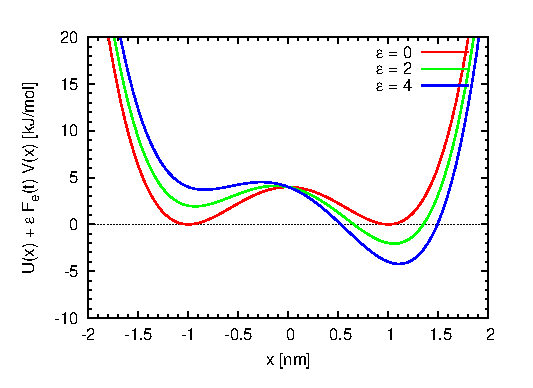
\includegraphics[width=0.4\textwidth]{figs/fig-tilt-pot.eps}
  \caption{The double-well potential with tilting perturbation at
    time $t\geq 20$ ps..}
  \label{fig:tmp1}
\end{figure}

\begin{figure}
  \centering
  \includegraphics[width=0.95\textwidth]
  {figs/fig-tilt-str2-2d-more.eps}
  \caption{The plot of $\Delta\mt_\tau f(\vect x,t)$ under
    perturbation with strength $\eps = 2$.  From left to right the
    columns present results at time $t = 0$, 10, 15 and
    20~\textsf{ps}.  The 1st row: the direct non-equilibrium
    simulation. The 2nd row: the results of traditional equilibrium
    linear response theory.  The 3rd row: the results of the response
    theory developed by this work.  We calculate response terms up to
    the second order from an equilibrium simulation (i.e. letting $k_0
    = 0$ and $\eps = 0$ in Eq.~\eqref{eqn:langevin-2b}).
  }
  \label{fig:tmp2}
\end{figure}

\begin{figure}
  \centering
  \includegraphics[width=0.95\textwidth]
  {figs/fig-tilt-str4-2d-more.eps}
  \caption{The plot of $\Delta\mt_\tau f(\vect x,t)$  under perturbation of
    $\eps = 4$. From left to right the
    columns present results at time $t = 0$, 10, 15 and
    20~\textsf{ps}.
    The first three rows use the same algorithm as Fig.~\ref{fig:tmp2}.    
    The 4th row: the results of the response theory developed by this work.
    Instead of calculating the responses from the equilibrium simulation,
    here we calculate the linear response from a non-equilibrium simulation
    of strength 2 (i.e. $k_0 = 2$ and $\eps = 4$
    in Eq.~\eqref{eqn:langevin-2b}).
    Therefore, the effective perturbation in this case is only
    $\eps = 2$.
  }
  \label{fig:tmp3}
\end{figure}

We test the idea firstly by a one-dimensional model system: one particle in a
tilting double-well potential. For convenience, we let the mass of the
particle to be 1~\textsf{amu},
and the friction coefficient to be $1\,\textsf{ps}^{-1}$.
The unperturbed
Hamiltonian of the system is given by:
\begin{align}
  \mh (\vect p, \vect q) = \frac 12 \vect p^2 + U(\vect q) 
\end{align}
with potential
\begin{align}
  U(\vect q) = \frac12 k (\vect q^2 - a^2)^2
\end{align}
Here $k = 8$~$\textsf{kJ} / (\textsf{mol nm}^4)$, and $ a = 1\ \textsf{nm}$.
At room temperature $300\ \textsf{K}$, $k_BT = 2.48$~\textsf{kJ/mol}.
The red line in Fig.~\ref{fig:tmp1} presents the unperturbed potential.
%$\textsf{kJ} / (\textsf{mol nm}^4)}$
The perturbation is given by
\begin{align}
  \vect D(\vect q) = -\nabla_{\vect q} V(\vect q) = 1
\end{align}
Here $V(\vect q) = -\vect q$   effectively tilts the original
potential $U(\vect q)$ (see the gree and blue lines in Fig.~\ref{fig:tmp1}).
The strength of $F_e(t)$ is
set to be 1, when the time $t$ is larger than some warm-up time $t_c$.
When $t \leq t_c$, the strength of $F_e(t)$ is linearly growing,
i.e. $ F_e(t) = t/t_c$.
We use the value $t_c = 20$~\textsf{ps}, so that the perturbation increases slow
enough: the typical decaying time scale of the correlation function
in~\eqref{eqn:eq-lr} is roughly 3~\textsf{ps}.
We choose $\tau = 1$~\textsf{ps}, and
% We choose $\mt_\alpha$
% to be the propagator of the Langevin dynamics at temperature $150$
% \textsf{K} with $\alpha = 1$ \textsf{ps}.
consider the stability of the
distribution $f(\vect x, t)$ at time $t$: $\Delta\mt_\tau f(\vect x, t)$.
The larger
this value, the more stable the core sets are.

See Fig.~\ref{fig:tmp2} and \ref{fig:tmp3} for numerical result.  Both
the results of the brute-force non-equilibrium simulation
and that of the response theory are presented.
In Fig.~\ref{fig:tmp2},
the good agreement between the brute-force (1st row)
and the linear response result (2nd row) indicates that $\eps = 2$ is
indeed a relatively small perturbation to the equilibrium.
In the third row of Fig.~\ref{fig:tmp2},
the second order response is considered. We do not see any
substantial improvement of the result by including this higher order term,
because the
driving force to the system is small,
and the linear term is anyway a good approximation.

In Fig.~\ref{fig:tmp3}, as the
perturbation grows stronger, the left well becomes less stable, while
the right well becomes more stable.  When the perturbation is as strong as
$\eps = 4$, the linear response result (2nd row) is no
longer precise:
At $t\geq 20$ \textsf{ps}, the left well basically
disappears, however, the linear response calculation presents
artificial structure (that is a small artificial
stable region accompanied by a small unstable region)
at the position of the left well.
The second order response (3rd row) improves the accuracy a little, 
however, it also includes artificial finer-grained oscillation in the profile.
At the same time, the numerical uncertainty is higher, so the figure
looks noisy.
In the 4th row of Fig.~\ref{fig:tmp3}, we present the linear response result
that calculate from 
a intermediate
non-equilibrium simulation with driving force of $k_0 = 2$.
Notice that the reference simulation in this case is also a
non-equilibrium simulation, so the effective strength of perturbation
is reduced to $\eps = 2$. According to Fig.~\ref{fig:tmp1}, this can be
considered as a small perturbation.
A substantial improvement is achieved: the profile
is correctly calculated, and the statistical error is small.

% the 1st order result of the
% response formula~\eqref{eqn:pert-approx-1} and
% \eqref{eqn:pert-approx-2}, with
% respect to the reference state $F_e^{\textrm{max}} = 2$. The result
% is impressively improved compared with the linear response with respect to the
% equilibrium state.


\subsection{Splitting single-well potential}

\begin{figure}
  \centering
  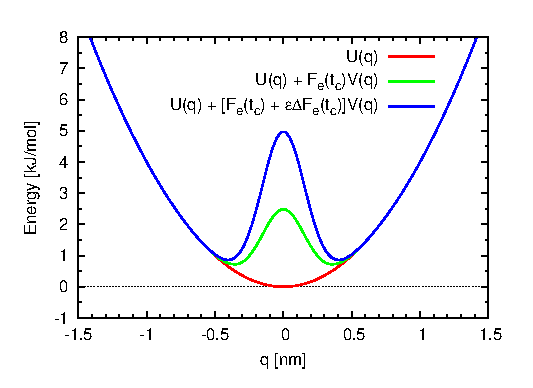
\includegraphics[width=0.4\textwidth]{figs/fig-split-pot.eps}
  \caption{The single-well potential with splitting perturbation at
    time $t\geq 20$ ps.}
  \label{fig:tmp4}
\end{figure}

% \begin{figure}
%   \centering
%   \includegraphics[width=0.95\textwidth]
%   {figs/fig-split-str1-2d-more.eps}
%   \caption{The plot of $\Delta\mt_\tau f(\vect x,t)$  under perturbation of
%     $F_e^{\textrm{max}} = 1.0$.
%     The 1st row: the direct non-equilibrium
%     simulation. The 2nd row: the results of linear response
%     formula~\eqref{eqn:core-identify-approx-2}.
%     The 3rd row: the results of response
%     formula~\eqref{eqn:pert-approx-1} and \eqref{eqn:pert-approx-2}.
%     The order is 2, the reference state is $F_e^{\textrm{max}} = 0$, i.e.
%     the equilibrium state.
%   }
%   \label{fig:tmp5}
% \end{figure}

\begin{figure}
  \centering
  \includegraphics[width=0.95\textwidth]
  {figs/fig-split-str2-2d-more.eps}
  \caption{
    The plot of $\Delta\mt_\tau f(\vect x,t)$  under perturbation of
    $\eps = 2$. From left to right the
    columns present results at time $t = 0$, 5, 10 and
    20~\textsf{ps}.
    The 1st row: the direct non-equilibrium
    simulation. The 2nd row: the results of traditional equilibrium
    linear response theory.  The 3rd row: the results of the response
    theory developed by this work.  We calculate response terms up to
    the second order from an equilibrium simulation (i.e. letting $k_0
    = 0$ and $\eps = 2$ in Eq.~\eqref{eqn:langevin-2b}).
    The 4th row: the results of the response theory developed by this work.
    Instead of calculating the responses from the equilibrium simulation,
    here we calculate the linear response from a non-equilibrium simulation
    of strength 2 (i.e. $k_0 = 1$ and $\eps = 1$
    in Eq.~\eqref{eqn:langevin-2b}).
    Only the linear term of response is calculated.
    Notice, the effective perturbation in this case is only
    $\eps = 1$.
  }
  \label{fig:tmp6}
\end{figure}

In the previous subsection, we considered an example that the stability of the
core sets is switched by an external driving to the system.
In this section, we consider ``splitting single-well potential'' example
that two new core sets grows out of 
an old core sets by the external driving force.
In this example, the unperturbed
potential is simply the harmonic potential given by:
\begin{align}
  U(\vect q) = \frac12\,k\,\vect q^2 
\end{align}
Here $k = 8$~$\textsf{kJ} / (\textsf{mol nm}^2)$.
See the red line in Fig.~\ref{fig:tmp4} for the unperturbed potential.
%$\textsf{kJ} / (\textsf{mol nm}^4)}$
The perturbation has again given by
\begin{align}
  \vect D(\vect q) = -\nabla_{\vect q} V(\vect q) 
\end{align}
where $V(\vect q)$ has a Gaussian profile:
\begin{align}
  V(\vect q) = \frac{1}{\sqrt{2\pi \sigma^2}}
  \exp\Big\{-\frac{\vect q^2}{2\sigma^2}\Big\}
\end{align}
we use $\sigma = 0.16$~\textsf{nm}.

In this example, we also consider two different strengths of
perturbations. Please see the green and blue lines in Fig~\ref{fig:tmp4} for
perturbations of $\eps = 1$ and $\eps = 2$, respectively.
Numerical results show that the perturbation $\eps=1$ can be considered to be
relatively small. Since the phenomenon is basically the same as
Fig.~\ref{fig:tmp2}, we do not present them here.
Fig.~\ref{fig:tmp6} presents the numerical results of perturbation $\eps =
2$.  Only with a linear response calculated from the equilibrium
simulation (2nd row), the stability of the two new core sets are too
strong, and the unstable region between them is over estimated, comparing with
the brute force simulation presented on the first row.
We present the  second order response results on the 3rd row, which is
also calculated from the equilibrium simulation. In this case, the statistical
error is too large, so that
the profile of $\mt_\tau f$ is indeed too noisy to draw any useful information.
On the 4th row of Fig.~\ref{fig:tmp6} presents the linear response starting
from a non-equilibrium simulation with external driving $k_0 = 1$.
In this case the effective strength of the perturbation to the reference
simulation is $\eps = 1$, which is considered to be relatively small.
The numerical results is satisfactorily consistent with the brute force
non-equilibrium simulation.



\section{Conclusions and Remarks}

When the strength of the perturbation $\eps$ is relatively small, then
the traditional linear response theory gives good approximation.  When
the perturbation reaches the strength, that is not small for the
linear response, including the second order response term does not
substantially improve the accuracy.
In the splitting single-well example, the statistical
noise of the second order response is so big that overwhelms the
information. Spending more computational effort on reducing the noise
is not economic. The non-equilibrium response theory developed by this
work allows one to calculate the response from some intermediate
non-equilibrium simulation, so the effective perturbation is much
smaller than it would be calculated from an equilibrium
simulation.
In both examples considered by this paper, the
numerical results of the proposed idea  satisfactory consistent with the
brute force non-equilibrium simulation.
From the face that, in a strongly driven system,
one should do an intermediate non-equilibrium
simulation and calculate the response from it,
one may argue that this may not be able to
save a lot computational cost comparing with a brute force
non-equilibrium simulation.  However, in practice, one need the
response theory for the following reasons: (1) One may want to study
multiple non-equilibrium system that are not very far from each other,
so only do one system and apply the linear response idea takes
advantage over doing non-equilibrium simulation for each of them.
(2) A stronger driven non-equilibrium system may be more difficult to
simulation directly comparing with a weakly driven system. For
example, the energy barrier between two rare events may be increased
greatly due to the external driven. (3) By the traditional linear
response theory, some information concerning the intermediate
non-equilibrium system can be derived from an standard equilibrium
simulation.
With this extra information, may be able to design better simulation methods
for the intermediate non-equilibrium system,
so that it is not as expensive as a brute force non-equilibrium
simulation starting with nothing know before hand.
(4) A thermodynamic multistep integration method can be developed from the
response theory plus idea (3): the non-equilibrium driving is increased
step-by-step and the total simulation effort at all the steps is still
cheaper than doing one brute force non-equilibrium simulation for the
target driven system.
Till now we have not investigated idea (3) and (4) mentioned above,
however, we believe the non-equilibrium response theory is a very
important step toward it and by itself deserves a separate careful
investigation.








% \newpage
% \section{Numerical results}
% \subsection{Tilting double-well potential}

% \begin{figure}
%   \centering
%   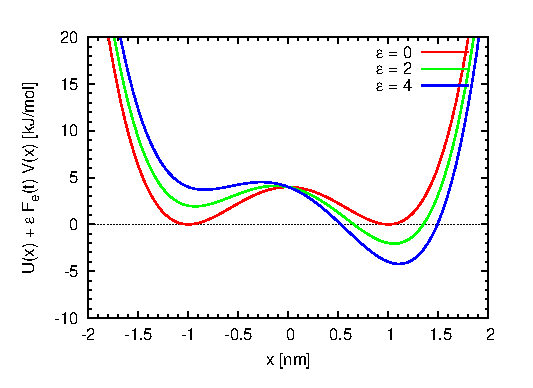
\includegraphics[width=0.4\textwidth]{figs/fig-tilt-pot.eps}
%   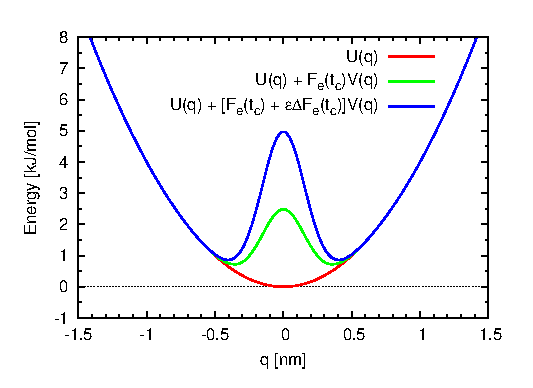
\includegraphics[width=0.4\textwidth]{figs/fig-split-pot.eps}
%   \caption{Two testing cases presented by this paper.
%     Left: the double-well potential with tilting perturbation.
%     Right: the single-well potential with splitting perturbation.}
%   \label{fig:new-tmp1}
% \end{figure}


% We test the idea by a one-dimensional model system: one particle in a
% tilting double-well potential. For convenience, we let the mass of the
% particle to be 1 \textsf{amu}. The unperturbed
% Hamiltonian of the system is given by:
% \begin{align}
%   \mh (\vect p, \vect q) = \frac 12 \vect p^2 + U(\vect q) 
% \end{align}
% with potential
% \begin{align}
%   U(\vect q) = \frac12 k (\vect q^2 - a^2)^2
% \end{align}
% Here $k = 8$~$\textsf{kJ} / (\textsf{mol nm}^4)$, and $ a = 1\ \textsf{nm}$.
% Notice at room temperature $300\ \textsf{K}$, $k_BT = 2.48$~\textsf{kJ/mol}.
% See the red line in Fig.~\ref{fig:tmp1}.
% %$\textsf{kJ} / (\textsf{mol nm}^4)}$
% The perturbation is given by
% \begin{align}
%   \vect C(\vect p, \vect q) = 0; \qquad
%   \vect D(\vect p, \vect q) = -\nabla_{\vect q} V(\vect q) = 1
% \end{align}
% Here $V(\vect q) = -\vect q$ is  effectively tilting the original
% potential $U(\vect q)$. The strength of the perturbation $F_e(t)$ is given
% by the following function:
% \begin{align}
%   F_e(t) = 
%   \begin{cases}
%     F_e^{\textrm{max}}\times (t / t_c) & t < t_c \\
%     F_e^{\textrm{max}} & t \geq t_c
%   \end{cases}
% \end{align}
% $t_c = 20$~\textsf{ps} so that the perturbation increases slow
% enough: the typical decaying time scale of the correlation function
% in~\eqref{eqn:core-identify-approx-2} is roughly 3~\textsf{ps}.
% We choose $\tau = 1$~\textsf{ps}.
% % We choose $\mt_\alpha$
% % to be the propagator of the Langevin dynamics at temperature $150$
% % \textsf{K} with $\alpha = 1$ \textsf{ps}.
% Since the dynamics is in
% 1-d, the projection $\mathcal P$ is identity.  We consider the stability of the
% distribution $f(\vect x, t)$ at time $t$: $\Delta\mt_\tau f(\vect x, t)$.
% The larger
% this value, the more stable the core sets are.

% \begin{figure}
%   \centering
%   \includegraphics[width=0.95\textwidth]
%   {figs/fig-tilt-str2-simple.eps}
%   \caption{
%     Tilting double well potential testing case:
%     the plot of $\Delta\mt_\tau f(\vect x,t)$  under perturbation of
%     $F_e^{\textrm{max}} = 2.0$.
%     From left to right:
%     (a) $t=0$~\textsf{ps},
%     the brutal force non-equilibirum simulation,
%     (b) $t=20$~\textsf{ps},
%     the brutal force non-equilibirum simulation,
%     (c) $t=20$~\textsf{ps},
%     response formula truncated at order $n=1$,
%     and
%     (d) $t=20$~\textsf{ps},
%     response formula truncated at order $n=2$.
%     The equilibirum state serves as the reference of
%     the response simulations.
%   }
%   \label{fig:new-tmp2}
% \end{figure}


% \begin{figure}
%   \centering
%   \includegraphics[width=0.95\textwidth]
%   {figs/fig-tilt-str4-simple.eps}
%   \caption{
%     Tilting double well potential:
%     the plot of $\Delta\mt_\tau f(\vect x,t)$  under perturbation of
%     $F_e^{\textrm{max}} = 4.0$.
%     From left to right:
%     (a) $t=0$~\textsf{ps},
%     the brutal force non-equilibirum simulation,
%     (b) $t=20$~\textsf{ps},
%     the brutal force non-equilibirum simulation,
%     (c) $t=20$~\textsf{ps},
%     response formula with reference process $F_e^{\max} = 0.0$
%     (i.e. equilibirum simulation),
%     and
%     (d) $t=20$~\textsf{ps},
%     response formula with reference process $F_e^{\max} = 2.0$.
%     The response formula are truncated at order $n=1$.
%   }
%   \label{fig:new-tmp3}
% \end{figure}



% The Fig.~\ref{fig:new-tmp2} and \ref{fig:new-tmp3} present
% the application of the response theory to
% calculate core sets of the tilting double-well potential.
% Fig.~\ref{fig:new-tmp2} presents
% the snapshot at $t=20$~\textsf{ps}
% of $\Delta\mt_\tau f(\vect x,t)$ under the maximum perturbation
% strength $F_e^{\max} = 2.0$. Response formula truncated
% at both order $n=1$ and $n=2$ are compared to 
% the brutal force non-equilibirum simulation.
% No obviously difference is shown. The second order response result
% is slightly more precise than the first order one, but the
% statistical error is also larger, which makes the profile noisy.
% This figure tells us that
% (1) the modeling error of the linear response (1st order) is
% negligibly small; (2) the statistical error of numerically measuring the
% linear response is also small.
% Fig.~\ref{fig:new-tmp3} presents the $t=20$~\textsf{ps}
% snapshots of $\Delta\mt_\tau f(\vect x,t)$
% under a larger perturbations $F_e^{\max} = 4.0$.
% The linear reponse using the equilibirum process as the reference
% shows poor accuracy: the left well vanishes in this case,
% while the linear response produces  artifical structures.
% Since the profile is smooth, which indicates
% the statistical error of calculating the linear term is small,
% the deviation comes from the modellng error, namely the contribution
% of higher order response terms.
% By including the second order response term reduces the left
% artifical core set, but also creates artifical finer grained
% structures. The statistical accuracy is also worse than the linear response.
% Plot (d) present the result of the linear response
% formula using reference process $F_e^{\max} = 2.0$, which
% is the process presented in Fig.~\ref{fig:new-tmp2}.
% Much better modelling accuracy is achieved:
% the left artifical core set disappear and the
% statistical accuracy is also satisfactory.

% % See Fig. \ref{fig:tmp2} and \ref{fig:tmp3} for numerical result.  Both
% % the direct non-equilibrium simulation and the response
% % approximations are presented. Time slices $t = 0$, 10, 15 and 20
% % \textsf{ps} are shown.  When the perturbation is small,
% % i.e. $F_e^{\textrm{max}} = 2$, the direct non-equilibrium simulation
% % and the linear response results are accurately consistent.
% % The 2nd order response formula~\eqref{eqn:pert-approx-1} and
% % \eqref{eqn:pert-approx-2} are even better, but the numerical error
% % is bigger.
% % As the
% % perturbation grows stronger, the left well becomes less stable, while
% % the right well becomes more stable.  When the perturbation is big,
% % i.e. $F_e^{\textrm{max}} = 4$, the linear response result is no
% % longer precise.
% % When $t\geq 20$ \textsf{ps}, the left well basically
% % disappears, however, the linear response calculation presents
% % artifical occilation at the right well.
% % The 2nd order response also has artifical effect, and the numerical
% % uncertainty is high.
% % The 4th rwo of Fig.~\ref{fig:tmp3} presents the 1st order result of the
% % response formula~\eqref{eqn:pert-approx-1} and
% % \eqref{eqn:pert-approx-2}, with
% % respect to the reference state $F_e^{\textrm{max}} = 2$. The result
% % is impressively improved compared with the linear response with respect to the
% % equilibrium state.




% \subsection{Splitting single-well potential}

% In this splitting single-well potential example, the unperturbed
% potential is simply the harmonic potential given by:
% \begin{align}
%   U(\vect q) = \frac12\,k\,\vect q^2 
% \end{align}
% Here $k = 8$~$\textsf{kJ} / (\textsf{mol nm}^2)$.
% Notice at room temperature $300\ \textsf{K}$, $k_BT = 2.48$~\textsf{kJ/mol}.
% See the red line in Fig.~\ref{fig:tmp4}.
% %$\textsf{kJ} / (\textsf{mol nm}^4)}$
% The perturbation is again given by
% \begin{align}
%   \vect C(\vect p, \vect q) = 0; \qquad
%   \vect D(\vect p, \vect q) = -\nabla_{\vect q} V(\vect q) 
% \end{align}
% where $V(\vect q)$ is a Gaussian type potential:
% \begin{align}
%   V(\vect q) = \frac{1}{\sqrt{2\pi \sigma^2}}
%   \exp\Big\{-\frac{\vect q^2}{2\sigma^2}\Big\}
% \end{align}
% we use $\sigma = 0.16$~\textsf{nm}. Please see Fig~\ref{fig:tmp4}.
% For the results, please see Fig.~\ref{fig:tmp5} -- Fig.~\ref{fig:tmp6}.




% \begin{figure}
%   \centering
%   \includegraphics[width=0.95\textwidth]
%   {figs/fig-split-str1-simple.eps}
%   \caption{
%     Splitting single-well potential testing case:
%     the plot of $\Delta\mt_\tau f(\vect x,t)$  under perturbation of
%     $F_e^{\textrm{max}} = 1.0$.
%     From left to right:
%     (a) $t=0$~\textsf{ps},
%     the brutal force non-equilibirum simulation,
%     (b) $t=20$~\textsf{ps},
%     the brutal force non-equilibirum simulation,
%     (c) $t=20$~\textsf{ps},
%     response formula truncated at order $n=1$,
%     and
%     (d) $t=20$~\textsf{ps},
%     response formula truncated at order $n=2$.
%     The equilibirum state serves as the reference of
%     the response simulations.
%   }
%   \label{fig:new-tmp5}
% \end{figure}


% \begin{figure}
%   \centering
%   \includegraphics[width=0.95\textwidth]
%   {figs/fig-split-str2-simple.eps}
%   \caption{
%     splitting single well potential:
%     the plot of $\Delta\mt_\tau f(\vect x,t)$  under perturbation of
%     $F_e^{\textrm{max}} = 2.0$.
%     From left to right:
%     (a) $t=0$~\textsf{ps},
%     the brutal force non-equilibirum simulation,
%     (b) $t=20$~\textsf{ps},
%     the brutal force non-equilibirum simulation,
%     (c) $t=20$~\textsf{ps},
%     response formula with reference process $F_e^{\max} = 0.0$
%     (i.e. equilibirum simulation),
%     and
%     (d) $t=20$~\textsf{ps},
%     response formula with reference process $F_e^{\max} = 1.0$.
%     The response formula are truncated at order $n=1$.
%   }
%   \label{fig:new-tmp6}
% \end{figure}







\section*{References}
\bibliography{ref}{}
\bibliographystyle{unsrt}





\end{document}